\chapter{System Architecture}
\section{Architecture}
The basic idea for this system to work was to use a pipe-and-filter architecture. We got some patient-cases and a medicine handbook, which should be used to search relevant ATC and ICD codes. Therefore, we had to first parse the patient-cases and handbook to be able to read and filter relevant words. 

\begin{figure}[h]
\centering
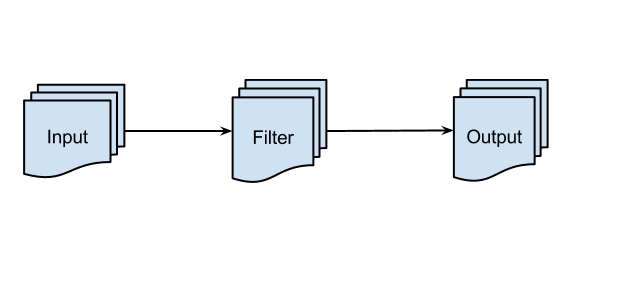
\includegraphics[scale=0.5]{system_architecture/architecture.png}
\caption{Basic idea of architecture}
\end{figure}

\pagebreak
\section{Components}

\begin{figure}[h]
\centering
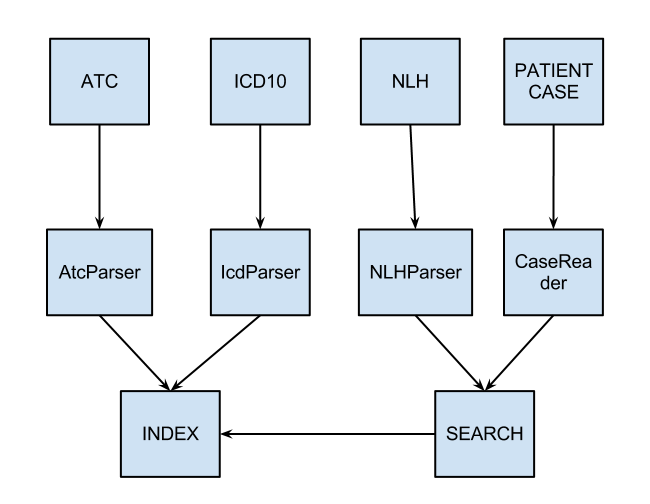
\includegraphics[scale=0.5]{system_architecture/components.png}
\caption{An overview of components}
\end{figure}

Our idea was to parse the atc- and icd-codes such that we could make an index of them both. After preprocessing the medicine handbook and patient cases we could take each sentence in them and use as a search query in the atc/icd indexes. Using Apache Lucene we got a ranked result of the best matching codes linked to every sentence. 

\begin{description}
\item{\textbf{ATC/AtcParser:}} \\
The atc was given as a prolog file. The ATC is used to read this prolog file so we could store it as atc-objects with help of the AtcParser.
\item{\textbf{Icd/IcdParser:}} \\
The icd-codes was given as an owl-file. Therefore we had to use Apache Digester to set rules for how to read and parse the owl-file. They were stored as icd-objects. 
\item{\textbf{NLH/NLHParser:}} \\
The norwegian medicine handbook was given as html-files. With help of the NLHParser we could strip each chapter for html-tags and then create a xml-file of that chapter. We did also strip the xml- files for stopwords and used a snowball stemmer(org.tartarus.snowball).
\item{\textbf{Patient-case:}} \\
The patient-cases was given in a doc-file. We extracted each case in own text-files. Then with help of the CaseReader we stripped the case for stopwords and stemmed it with help of the snowball stemmer. 
\item{\textbf{Index:}} \\
The indexer using Apache Lucene takes the atc-codes and index the label and code. The indexer for icd index the label, code and synonyms.This are then stored in resources/index/.. in the project so it can be accessed by the searcher. 
\item{\textbf{Search:}} \\
Now that the patient-cases and the handbook were in the same standard we wanted to do a search. The search takes each sentence from each patient-case and handbook chapter and search through the atc and icd codes for relevant hits. This was implemented with Apache Lucene so we could read the stored index for atc and icd. This allowing us to search in the index and Lucene will then give us ranked hits. 
\item{\textbf{vectorSpace package:}} \\
This package is the codification of the VSM. Here is a general overview of the classes and their functions:
\begin{description}
\item{textit{DocVector.java: }} \\
This class is used to make vectors out of (indexed) documents. It also has a DocCollection listener in order to avoid duplicates.
\item{textit{DocCollection.java: }} \\
This class creates a collection of documents(vectors), which is implemented as a hashmap. This class is updated every time we add another document(vector).
\item{textit{VectorSpace.java: }} \\
This class does the calculation of the cosine similarity. It calculates the cosine value between two documents(vectors).
\item{textit{VectorMain.java: }} \\
This class has only a comprehensive main method, which is the very finalization of the algorithm, since it does the ranking of the relevant documents. It uses all of the above mentioned classes.
\end{description}
\end{description}